\documentclass[final]{beamer}

\usepackage[size=custom,width=152,height=123]{beamerposter}
% \usepackage{wrapfig}
\usepackage{subcaption}

\usetheme{Pittsburgh}

\definecolor{orange}{RGB}{243,112,33}
\definecolor{blue}{RGB}{0,84,150}
\setbeamercolor{block title}{fg=orange,bg=white} % Colors of the block titles
\setbeamercolor{block body}{fg=black,bg=white} % Colors of the body of blocks
\setbeamercolor{block alerted title}{fg=white,bg=dblue!70} % Colors of the highlighted block titles
\setbeamercolor{block alerted body}{fg=black,bg=dblue!10} % Colors of the body of highlighted blocks
% Many more colors are available for use in beamerthemeconfposter.sty

%-----------------------------------------------------------
% Define the column widths and overall poster size
% To set effective sepwid, onecolwid and twocolwid values, first choose how many columns you want and how much separation you want between columns
% In this template, the separation width chosen is 0.024 of the paper width and a 4-column layout
% onecolwid should therefore be (1-(# of columns+1)*sepwid)/# of columns e.g. (1-(4+1)*0.024)/4 = 0.22
% Set twocolwid to be (2*onecolwid)+sepwid = 0.464
% Set threecolwid to be (3*onecolwid)+2*sepwid = 0.708

\newlength{\sepwid}
\newlength{\onecolwid}
\newlength{\twocolwid}
\newlength{\threecolwid}
\setlength{\paperwidth}{152cm} 
\setlength{\paperheight}{123cm} %
\setlength{\sepwid}{0.02\paperwidth} % Separation width (white space) between columns
%\setlength{\onecolwid}{0.3\paperwidth} % Width of one column
%\setlength{\twocolwid}{0.6\paperwidth} % Width of two columns
\setlength{\onecolwid}{0.225\paperwidth} % Width of one column
\setlength{\twocolwid}{0.47\paperwidth} % Width of two columns
\setlength{\threecolwid}{0.715\paperwidth} % Width of two columns
%\setlength{\topmargin}{-1.5in} % Reduce the top margin size
%-----------------------------------------------------------

\usepackage{qrcode}
\usepackage{graphicx}  % Required for including images
\graphicspath{./fig}

\usepackage{booktabs} % Top and bottom rules for tables


\begin{document}

\addtobeamertemplate{block end}{}{\vspace*{2ex}} % White space under blocks
\addtobeamertemplate{block alerted end}{}{\vspace*{2ex}} % White space under highlighted (alert) blocks

\setlength{\belowcaptionskip}{2ex} % White space under figures
\setlength{\belowdisplayshortskip}{2ex} % White space under equations

\begin{frame}[t] % The whole poster is enclosed in one beamer frame

%----------------------------------------------------------------------------------------
%	TITLE SECTION
%----------------------------------------------------------------------------------------
\rule{\textwidth}{0.2cm}
\begin{columns}
  \begin{column}{\sepwid}\end{column} % Empty spacer column
  % \begin{center}
  \begin{column}{\threecolwid}
    {\fontsize{130}{180}
        %\rule{\linewidth}{0.25cm}
        \textsc{%textsc makes text small capsx1%aQ$&kSPmV
        \color{orange}{A Topological Approach to Magnetic Nulls}}\\
    }
  \end{column}
  \begin{column}{\sepwid}\end{column} % Empty spacer column
  \begin{column}{1.2\onecolwid}
    \begin{large}
        \textsc{Ben Israeli$^{1,\dagger}$, Christopher Berg Smiet$^{1,2}$, Amitava Bhattacharjee$^{1}$}\\
        \color{orange}{$^1$Princeton Plasma Physics Laboratory, Princeton, 08540 NJ, USA},\\
        \color{orange}{$^2$Leiden University, Leiden, 2300 RA, Netherlands}\\
        \color{blue}{$^\dagger$ bisraeli@pppl.gov}
  \end{large}
  \end{column}
%  \end{center}
\end{columns}
\rule{\textwidth}{0.2cm}




%----------------------------------------------------------------------------------------


\begin{columns}[t]

\begin{column}{\sepwid}\end{column} % Empty spacer column

\begin{column}{\onecolwid} % The first column

%----------------------------------------------------------------------------------------
%	BACKGROUND
%----------------------------------------------------------------------------------------
\begin{block}{\huge{Introduction}}
	Three-dimensional magnetic nulls play an important role in astrophysical
	plasma physics and earth-based fusion concepts such as the FRC. 
	We present a novel method of conceptualizing the movement of these nulls by treating
        them as the convergence point of isotropes (iso=same, tropos = direction), lines in space
	along which the magnetic field points in the same direction. 
	It is shown that the isotropes can be recovered as the stream lines of
	the isotrope field, which is defined via a geometric formula from the
	magnetic field, and for which nulls act as charges analogous to point charges generating
        and electric field. In this way, the index theorem for magnetic nulls can be reframed as a Gauss's Law
        on the isotrope field. 
	
\end{block}

\begin{block}{\huge{Background}}
\begin{block}{Type A and Type B Nulls}
  Because magnetic fields are divergence free,
  nulls of 3D magnetic fields are constrained to be one of two types:
  \begin{columns}[t,totalwidth=\onecolwid] % Split up the two columns wide column
    \begin{column}{.45\onecolwid}
        \begin{centering}
        \textbf{Type A (Index -1)}
        \begin{figure}
        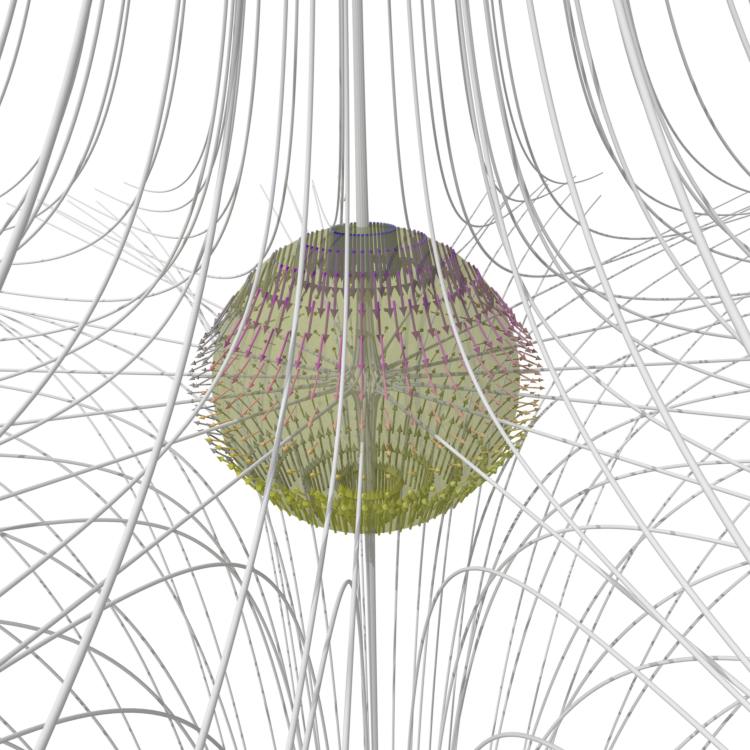
\includegraphics[width=.45\onecolwid]{fig/negindex_start.png}
        \end{figure}
        \end{centering}
    \end{column}

    \begin{column}{.45\onecolwid}
        \begin{centering}
        \textbf{Type B (Index +1)}
        \begin{figure}
        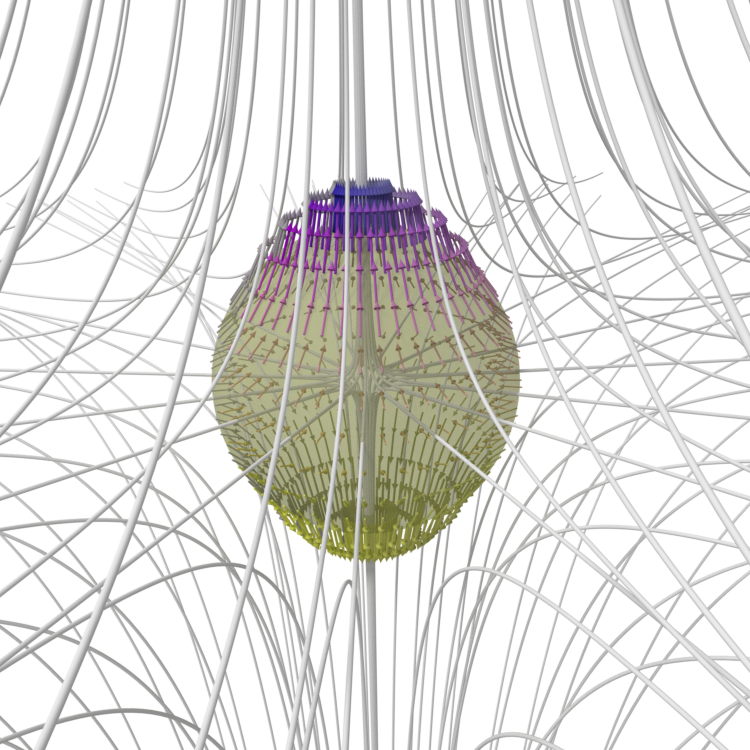
\includegraphics[width=.45\onecolwid]{fig/posindex_start.png}
        \end{figure}
    \end{centering}
    \end{column}
  \end{columns}
  
  %\fbox{
    %\footnotesize{
    %\begin{minipage}{\textwidth}
    \vspace{10pt}
    This can be understood via the eigenvalues of the Jacobian of the magnetic field at the null:
    \begin{equation}\label{eq:matrix}
        \mathsf{J}_{ij}= \partial_j B_i.
    \end{equation}
    $\nabla\cdot\mathbf{B}=0$ implies $\mathrm{Tr}(\mathsf{J})=0$. As a result, $J$ must have either all real
    eigenvalues or a pair of conjugate eigenvalues and one real eigenvalue.
    Generically, two eigenvalues will share a sign of their real part,
    and one will necessarily have opposite sign. The paired eigenvalues have eigenvectors
    that span a ``fan plane'' extending from the null,
    while the remaining eigenvector follows a ``spine'' passing through this plane at the null.\\
    \textbf{Type A} nulls are those with one positive real eigenvalue,
    and \textbf{type B} nulls are those with one negative real eigenvalue,
    with flows along the spine and fan correspondingly directed.
    %\end{minipage}
    %}}
\end{block}

\begin{block}{Topological Index}
  Define the map $g:\mathbb{R}^3\rightarrow S^2$ that sends points in
  space to the unit vectors in the direction of the field $\mathbf{B}$
  (i.e. points on the unit sphere).
  \begin{equation}\label{eq:director}
    g = \frac{\mathbf{B}(\mathbf{x})}{|\mathbf{B}(\mathbf{x})|}
  \end{equation}
  Note that on a sufficiently small sphere around a null, this map is 1-to-1,
  inside out for type A nulls and outside out for type B nulls.\\
  {\Large
    A:$
    \begin{array}{c}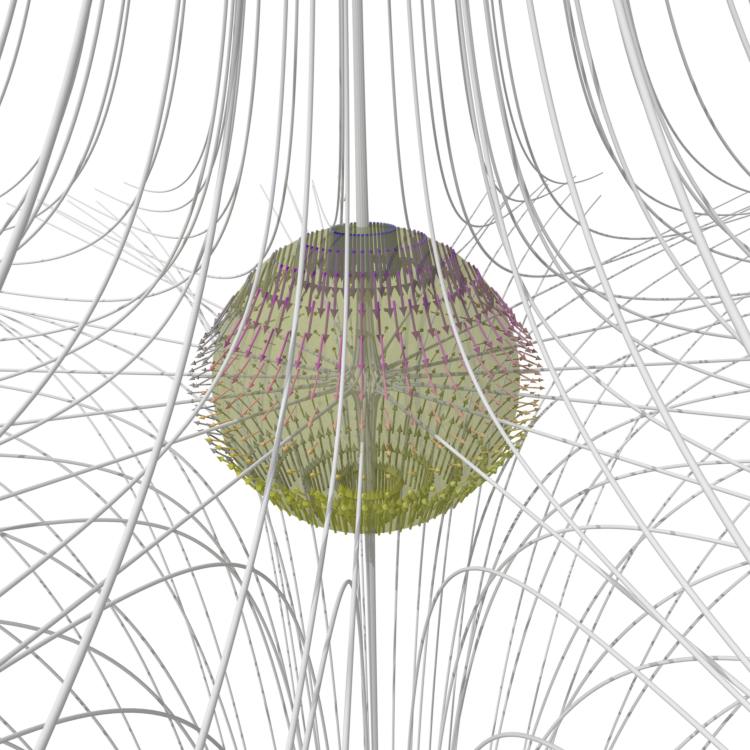
\includegraphics[width=.4\onecolwid]{fig/negindex_start.png}\end{array}
    \Rightarrow
    \begin{array}{c}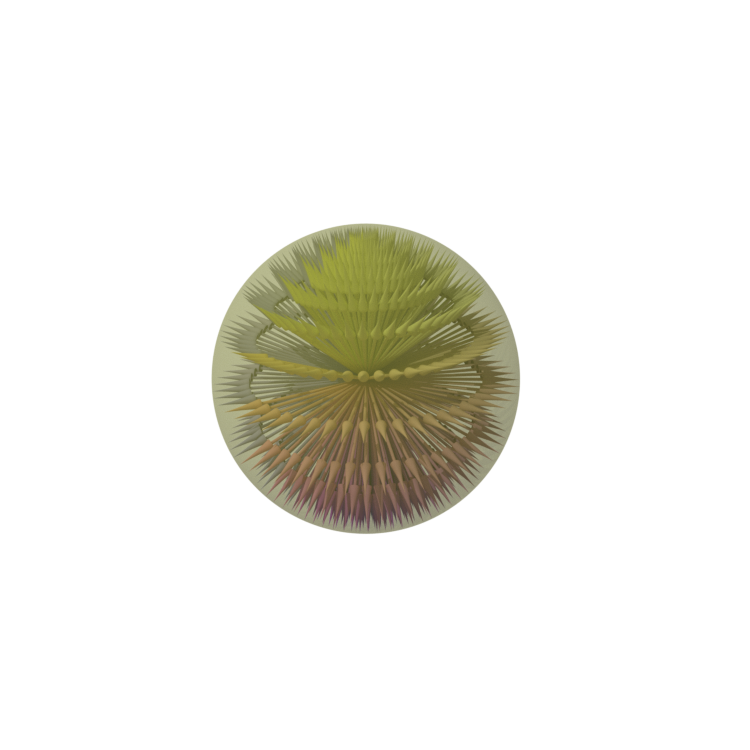
\includegraphics[width=.4\onecolwid]{fig/negindex_end.png}\end{array}
    $
    \\
    B:$
    \begin{array}{c}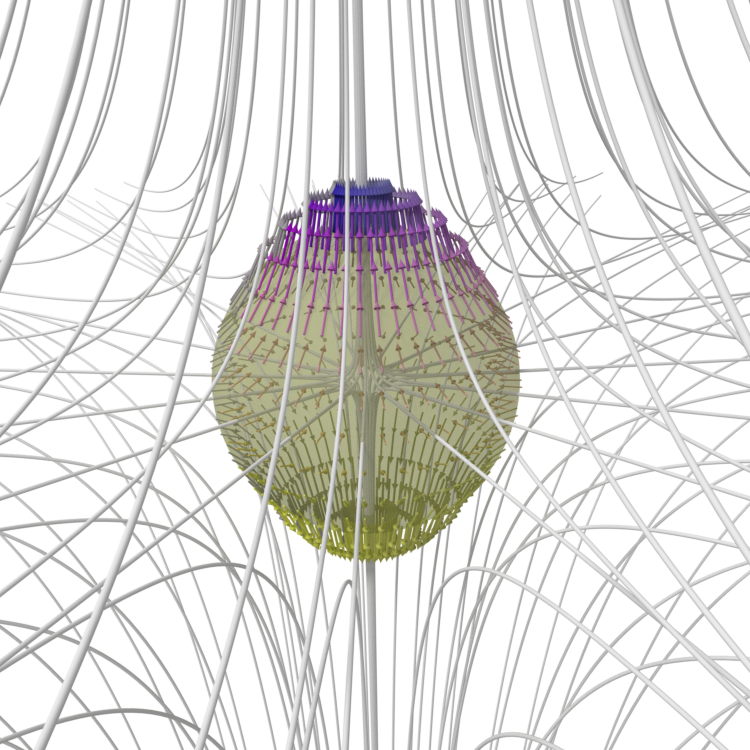
\includegraphics[width=.4\onecolwid]{fig/posindex_start.png}\end{array}
    \Rightarrow
    \begin{array}{c}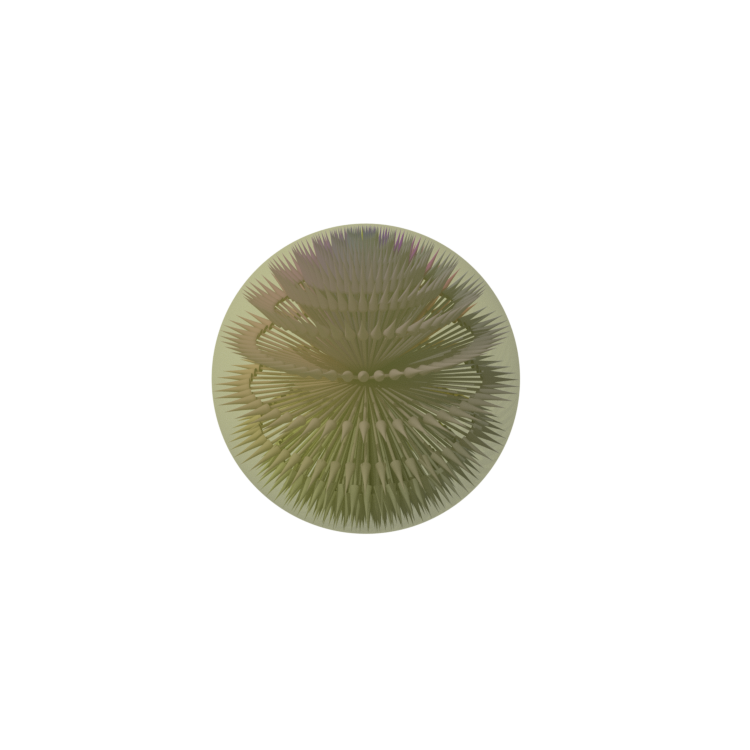
\includegraphics[width=.4\onecolwid]{fig/posindex_end.png}\end{array}
    $
  }\\
  The degree of a map is the number of times the domain wraps around the range.
  For the surface of a solid sphere containing a single null,
  the degree of the mapping $g|_{\partial D^3_{x_0}}$ is $-1$ for a type A null and $+1$ for a type B null.
  This is the \textbf{topological index} of an isolated null.
  \begin{equation}\label{eq:index1}
    \mathrm{Ind}(x_0)=\mathrm{Deg}(g|_{\partial D^3_{x_0}})
  \end{equation}
  The degree of any map between spheres is always in
  $\mathbb{Z}$~\cite{brouwer1911abbildung}, so $\mathrm{Deg}(g|_{\partial D^3})\in\mathbb{Z}$.
  If $D^3$ contains more than one isolated null, then the following theorem holds:
  {\Large
  \begin{equation}\label{eq:indextheorem}
    \boxed{\mathrm{Deg}(g|_{\partial D^3})= \sum_{x_0\in D^3} \mathrm{Ind}(x_0)}
  \end{equation}
  }
  The degree of the map counts the total topological index of the contained nulls.
\end{block}
\end{block}

%----------------------------------------------------------------------------------------

\end{column} % End first column

%----------------------------------------------------------------------------------------
%	ISOTROPES
%----------------------------------------------------------------------------------------

\begin{column}{\sepwid}\end{column} % Empty spacer column

\begin{column}{\onecolwid} % Begin the last column


%----------------------------------------------------------------------------------------
%
%----------------------------------------------------------------------------------------

\begin{block}{\huge{The Isotrope Field}}
\begin{block}{Isotrope Lines}
  The magnetic field direction defines a map from space to the sphere $g:\mathbb{R}^3\rightarrow S^2$,
  from a 3 dimensional manifold to a 2 dimensional manifold.
  Since this map loses a degree of freedom,
  at any point in $\mathbb{R}^3$ (with exeption of null points and singularities),
  there is a there is a direction in which the direction
  of the magnetic field remains constant.
  We call these lines the isotropes of the magnetic field.
  These lines cannot start or end, except at nulls.
  As described by the topological index of nulls, the magnetic field direction
  on a closed surface surrounding a single null takes on all possible values (mapping over all of $S^2$).
  Therefore any null is the termination of isotropes for every magnetic field direction.
\end{block}

\begin{block}{Motivitating the Isotrope Field}
  {\Large
  We see that nulls:
  \begin{itemize}
  \item can be counted by integration over an enclosing surface.
  \item function as sources and terminations for isotrope lines.
  \end{itemize}
  In analogy to electrostatic point charges,
  this suggests constructing a field tangent to the isotrope lines (E-field lines)
  that has a Gauss's Law for topological index (electric charge).
  }
\end{block}

\begin{block}{Deriving the Isotrope Field}
  We want to construct some vector field $v$ such that integrating it over a closed surface
  gives the total topological index of the enclosed nulls.
  {\large
  \begin{equation}
    \boxed{\int_{\partial U}v\cdot da=4\pi\sum_{x_i\in U}\mathrm{Ind}(x_i)}
  \end{equation}
  }
  Calculating total index by counting covers of $S^2$ by the surface of a region $U\in\mathbb{R}^3$
  can be written:
  \begin{equation}
    4\pi\sum_{x_i\in U}\mathrm{Ind}(x_i)=\int_{g_*\partial U}\omega
  \end{equation}
  where we have defined some properly normalized area two-form $\omega$ on $S^2$.
  We need to transfer our notion of area on $S^2$ (defined by $\omega$)
  to an object that can be integrated over a surface in $R^3$.
  This is just the pull-back through our map $g:\mathbb{R}^3\rightarrow S^2$
  of the area two-form $\omega$:
  \begin{equation}
    4\pi\sum_{x_i\in U}\mathrm{Ind}(x_i)=\int_{\partial U}g^*\omega
  \end{equation}
  But we wanted a vector field, not a two-form, so we then take the Hodge dual:
  \begin{equation}
    v=\star g^*\omega
  \end{equation}
  which yields, as desired:
  \begin{equation}
    4\pi\sum_{x_i\in U}\mathrm{Ind}(x_i)=\int_{\partial U}v\cdot da
  \end{equation}
  Working with some arbitrary coordinates $(\alpha,\beta)$
  on $S^2$ with $\omega=d\alpha\wedge d\beta D(\alpha,\beta)$,
  we can derive the general form of $v$
  and verify it indeed lies tangent to the isotrope lines.
  \begin{equation}
    4\pi\sum_{x_i\in U}\mathrm{Ind}(x_i)
    =\int_{g_*\partial U}\omega
    =\int_{g_*\partial U}d\alpha d\beta D(\alpha,\beta)
    =\int_{\partial U}dxdy
    \begin{vmatrix}
      \partial_x\alpha & \partial_x \beta \\
      \partial_y\alpha & \partial_y \beta
    \end{vmatrix}
    D(\alpha,\beta)
    =\int_{\partial U}g^*\omega
    =\int_{\partial U}v\cdot da
  \end{equation}
  For any two vectors $a,b$:
  \begin{equation}
    v\cdot(a\times b)
    =g^*\omega(a,b)
    =\begin{vmatrix}
      \partial_a\alpha(\vec{x}) & \partial_a\beta(\vec{x}) \\
      \partial_b\alpha(\vec{x}) & \partial_b\beta(\vec{x})
    \end{vmatrix}
    D(\alpha(\vec{x}),\beta\vec{x}))
    =(\nabla\alpha\times\nabla\beta)\cdot(a\times b)D(\alpha,\beta)
  \end{equation}
  So $v$ can be written as:
  {\Large
  \begin{equation}
    \boxed{v=(\nabla\alpha\times\nabla\beta)D(\alpha,\beta)}
  \end{equation}
  }
  We can immediately see that $g:\vec{x}\mapsto (\alpha,\beta)$ is constant on streamlines of $v$, so the streamlines of $v$ are by definition the previously defined isotropes of $\mathbf{B}$.
  \begin{equation}
    v\perp\nabla\alpha,\nabla\beta\Rightarrow\partial_v\vec g=0
  \end{equation}
  If we choose to parameterize magnetic field direction with standard spherical coordinates,
  and use the usual solid angle definition of area on $S^2$, this becomes:
  \begin{equation}
    v=(\nabla\theta\times\nabla\phi)\sin\phi
  \end{equation}
  The isotrope field is directed away from nulls of index $+1$ and towards nulls of
  index $-1$.
  In this sense the isotrope field is analogous to the electric field of  point charges, and it's
  integral over a surface calculates the topological charge enclosed.
  \begin{columns}[t,totalwidth=\onecolwid] % Split up the two columns wide column
    \begin{column}{.45\onecolwid}
        \begin{centering}
        \textbf{Type A (Index -1)}
        \begin{figure}
        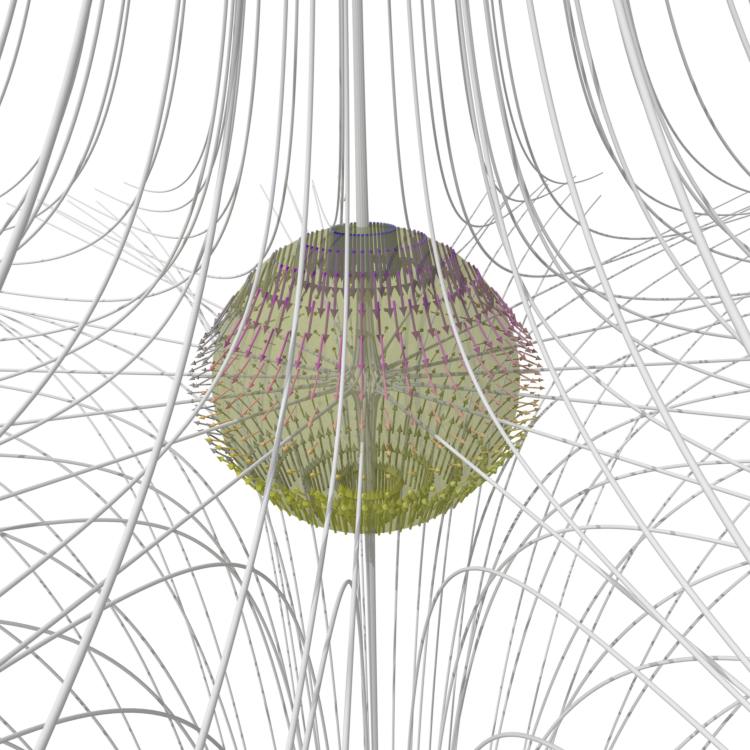
\includegraphics[width=.45\onecolwid]{fig/negindex_start.png}
        \end{figure}
        \end{centering}
    \end{column}

    \begin{column}{.45\onecolwid}
        \begin{centering}
        \textbf{Type B (Index +1)}
        \begin{figure}
        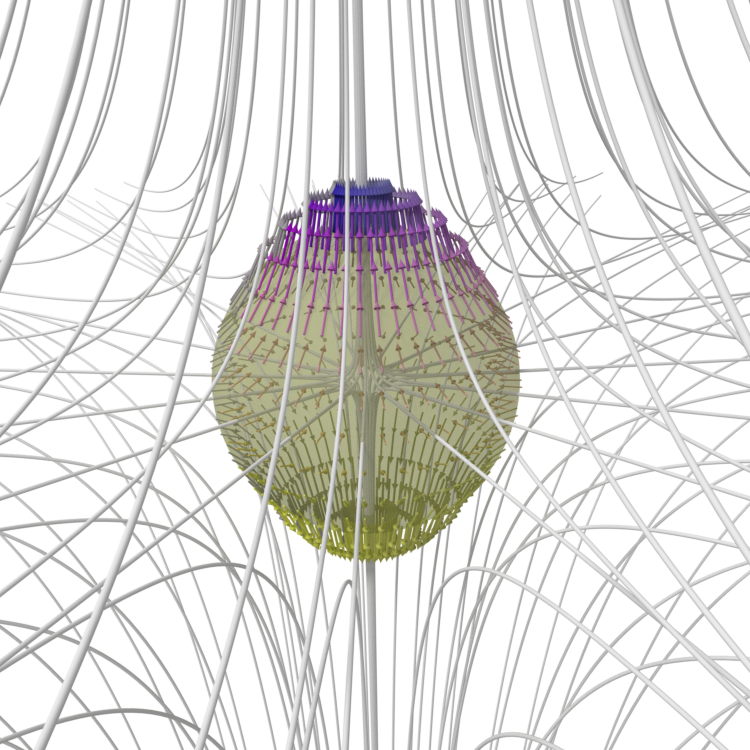
\includegraphics[width=.45\onecolwid]{fig/posindex_start.png}
        \end{figure}
    \end{centering}
    \end{column}
  \end{columns}
\end{block}

\end{block}
\end{column}


\begin{column}{\sepwid}\end{column} % Empty spacer column
%----------------------------------------------------------------------------------------
\begin{column}{\twocolwid} %Guide field section

\begin{block}{\huge{Local Magnetic Fields in Guide Fields}}

\begin{columns}[t,totalwidth=\twocolwid]

\begin{column}{\onecolwid}
\begin{block}{Isotropes of a Localized Field Embedded in a Guide Field}
  This work was motivated by the problem of determining the locations of nulls in a field generated by
  localized currents embedded in a homogeneous guide field
  and how these nulls move when the guide field is varied.
  \begin{itemize}
    \item Systems such as the magnetospheres of celestial objects and the field configuration in an FRC.
    \item Nulls appear on the isotrope (of the local field) corresponding with the direction opposite to the
      direction of the guide field,
      at its intersection with surfaces of constant field strength equalling that of the guide field.
    \item Sum of indices of all nulls must be 0.
    \item Isotrope pierces each surface of constant field strength twice(+1 on enterting, -1 on exiting).
   \end{itemize}
    
  \begin{figure}
    \centering
    \begin{subfigure}[b]{.45\textwidth}
      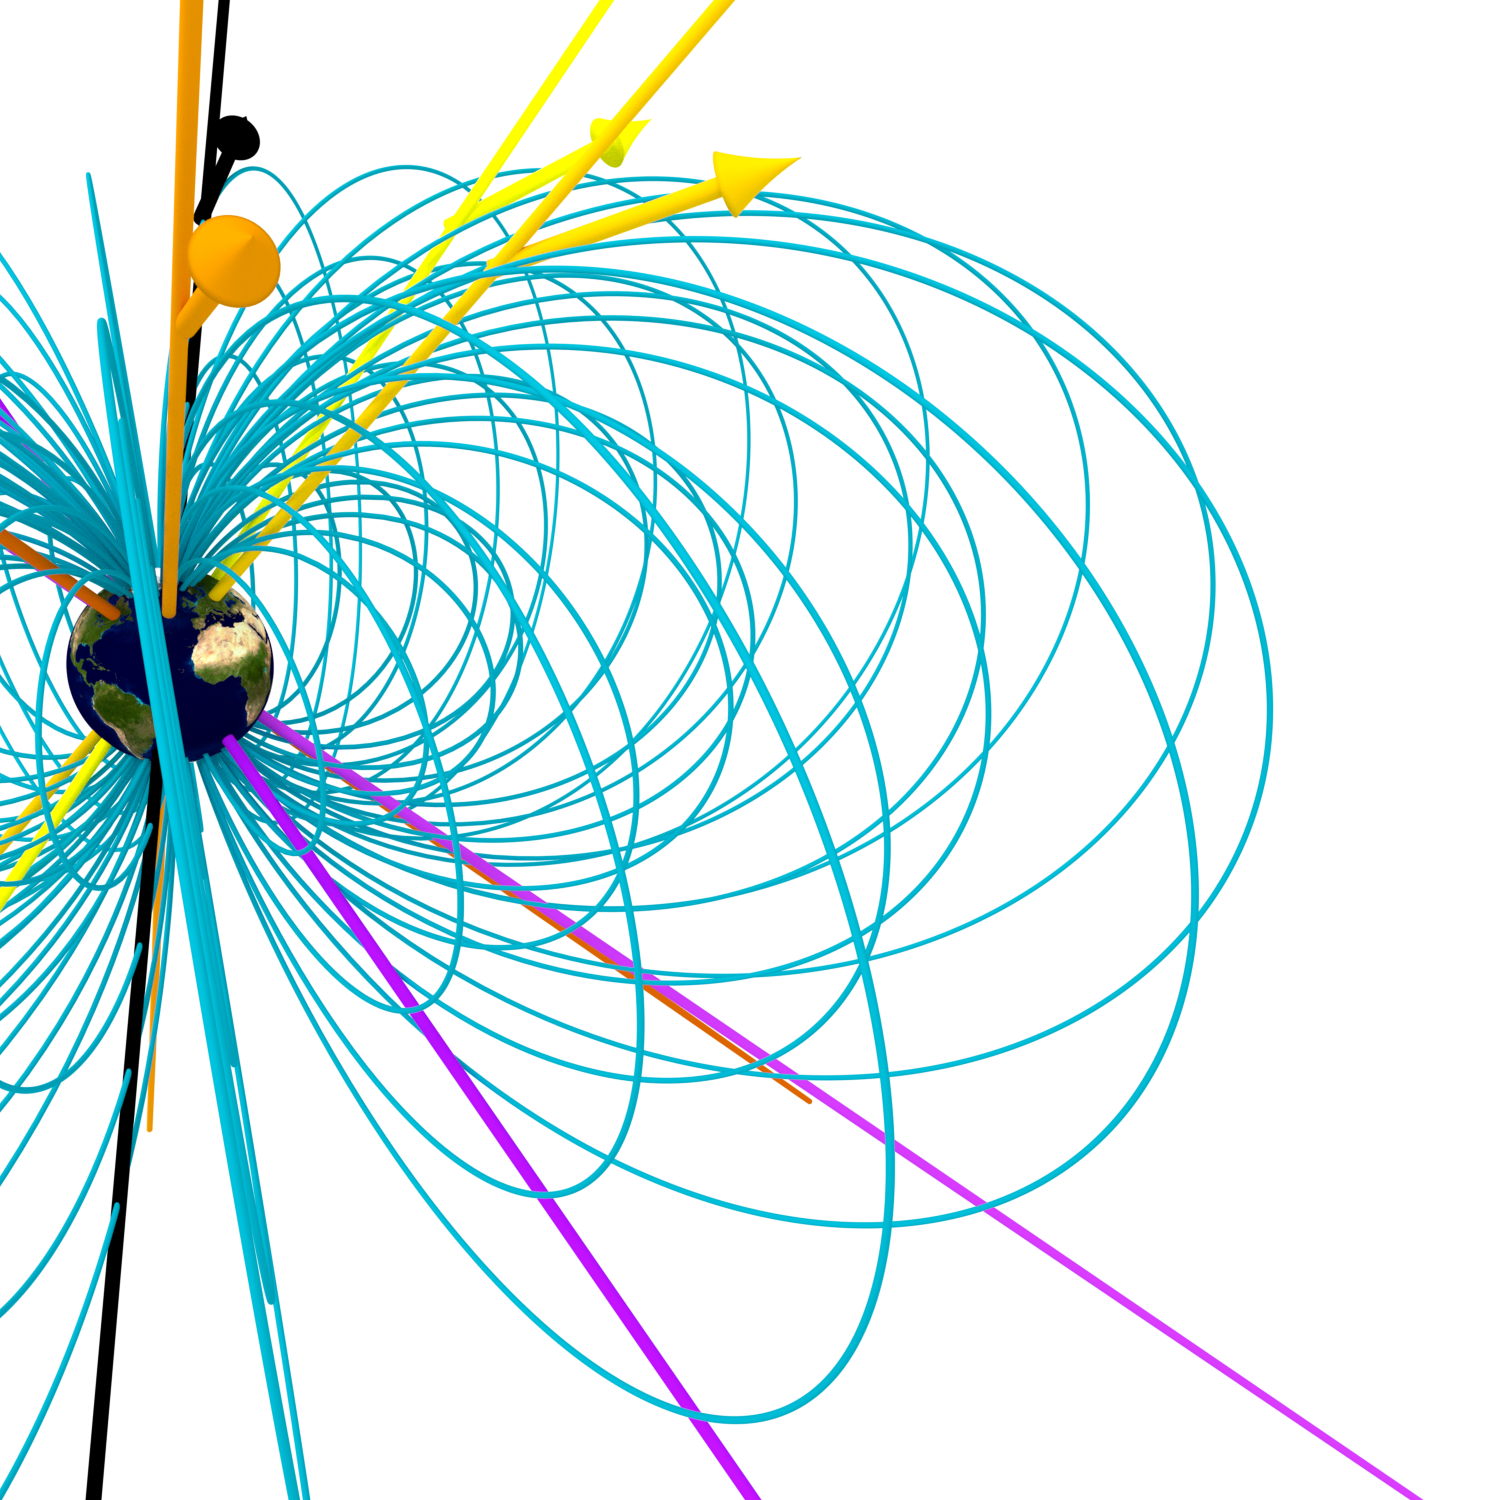
\includegraphics[width=\textwidth]{fig/mainfig.png}
      \caption{}
    \end{subfigure}
    \begin{subfigure}[b]{.45\textwidth}
      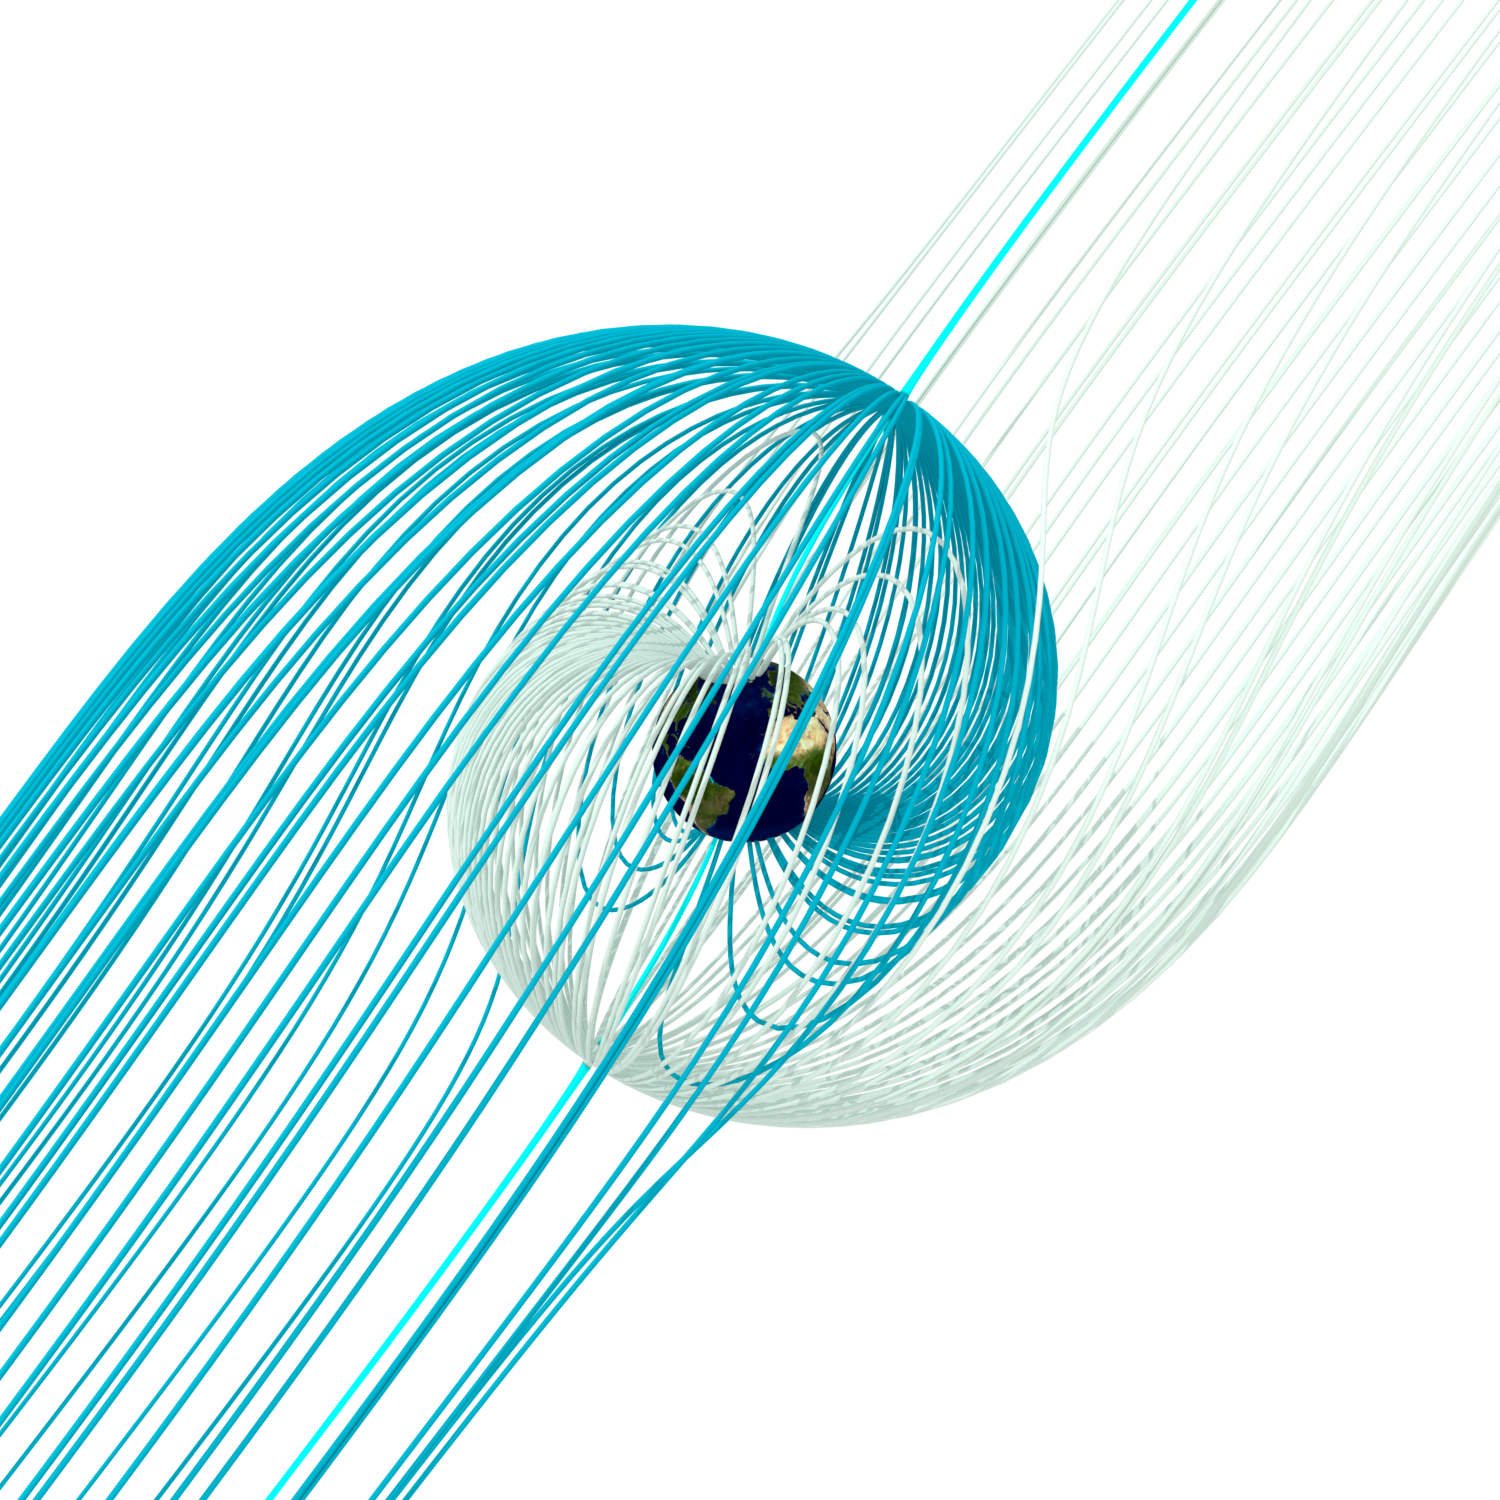
\includegraphics[width=\textwidth]{fig/separatrix_dipole.png}
      \caption{}
    \end{subfigure}
    \caption{
      a) The magnetic field of a dipole.
      The magnetic field lines are given by the blue curves.
      Seven isotropes are shown in different colors, with a vector indicating the diretion of the
      isotrope. b) The magnetic field of a dipole embedded in a guide field of direction $(-1,0,-1)$. 
      The spines are colored red, the fan corresponding to the
      index $-1$ null is dark blue and the fan corresponding to the
      index $+1$ is light blue.
    }
  \end{figure}
  \begin{figure}
    \centering
    \begin{subfigure}[b]{.45\textwidth}
      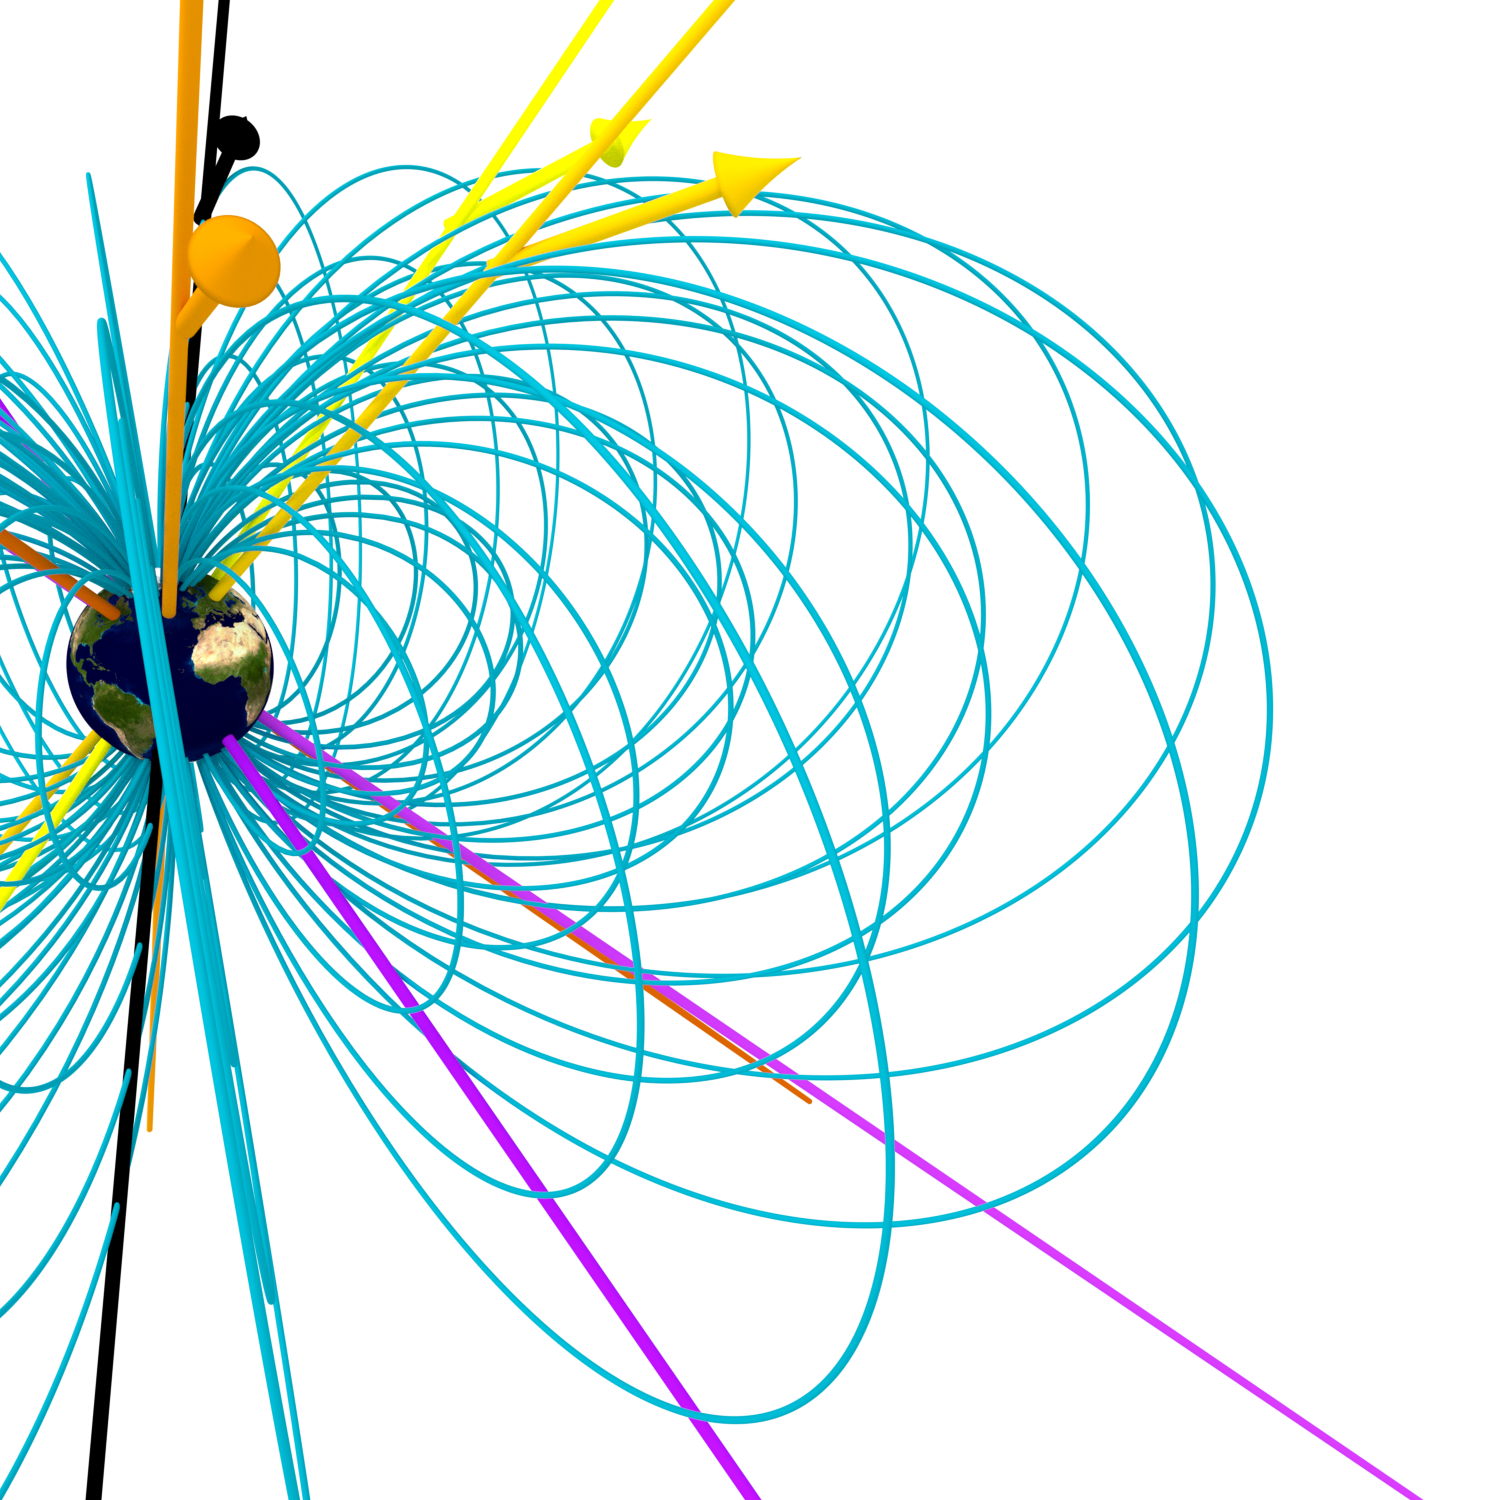
\includegraphics[width=\textwidth]{fig/mainfig.png}
      \caption{}
    \end{subfigure}
    \begin{subfigure}[b]{.45\textwidth}
      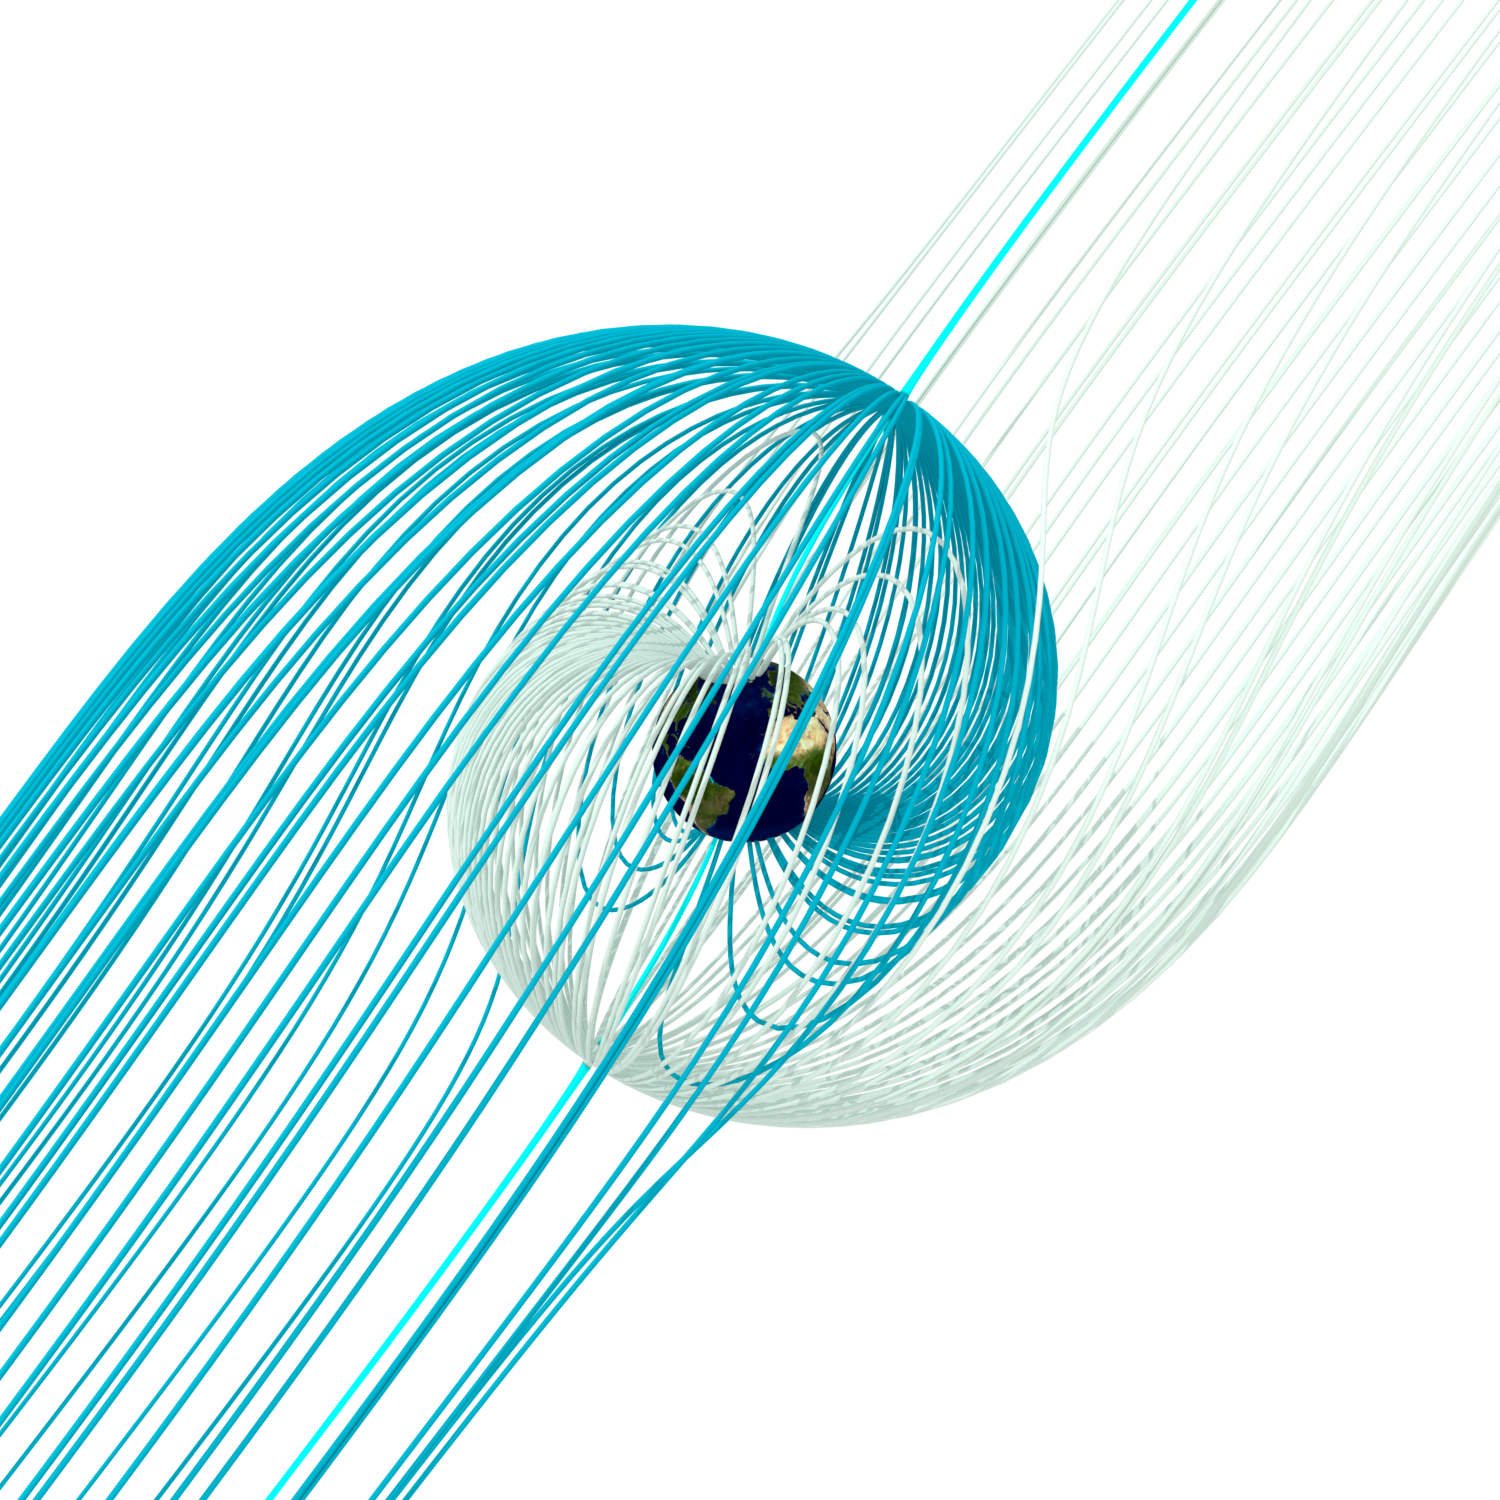
\includegraphics[width=\textwidth]{fig/separatrix_dipole.png}
      \caption{}
    \end{subfigure}
    \caption{
      a) The magnetic field of a dipole.
      The magnetic field lines are given by the blue curves.
      Seven isotropes are shown in different colors, with a vector indicating the diretion of the
      isotrope. b) The magnetic field of a dipole embedded in a guide field of direction $(-1,0,-1)$. 
      The spines are colored red, the fan corresponding to the
      index $-1$ null is dark blue and the fan corresponding to the
      index $+1$ is light blue.
    }
  \end{figure}
\end{block}
\end{column}
\begin{column}{\sepwid}\end{column} % Empty spacer column
\begin{column}{\onecolwid}
\begin{block}{Movement of Nulls}
  \begin{itemize}
    \item As the guide field is varied smoothly, the location of nulls changes smoothly.
    \item As guide field strength is varied, nulls move along the isotropes for the guide field direction.
    \item Nulls of opposite type move in opposite directions along isotropes,
      and can be annihilated/created where they meet.
  \end{itemize}
\end{block}

\begin{block}{Singular Surfaces of the Jacobian}
  \begin{itemize}
    \item The Jacobian $J$ of the magnetic field is independent of the (homogeneous) guide field,
      and therefore so are its eigenvalues.
    \item As a result, the system is split into regions (invariant w.r.t. the guide field) of $|J|\lessgtr 0$,
      where nulls of only one type or the other can appear.
    \item These are separated by surfaces (or regions) where $|J|=0$ and therefore $\nabla\times B=0$.
    \item As a guide field is varied, if a null drifts onto a singular surface, it necessarily annihilates
      against a null of opposite type from the other side.
    \item Conversely, nulls can only be created (by varying a guide field) in pairs at singular surfaces.
    \item $|B|$ reaches a local extremum along the path of an isotrope as it crosses a singular surface.
    \end{itemize}
\end{block}

\begin{block}{Nulls Near Singular Surfaces}
  \begin{itemize}
    \item Using the identities $J\cdot v=B v\cdot \nabla \ln|B|$ (globally) and $v\cdot \nabla |B|=0$ (at the surface), $J\cdot v=0$.
    \item The isotropic field is a zero eigenvector of $J$ at the singular surface.
    \item Eigenvectors and eigenvalues vary smoothly in $R^3$,
      so near the surface there is an eigenvector $~v$ for the eigenvalue that vanishes at the surface.
    \item On a path connection two nulls across a singular surface,
      the eigenvalue that changes sign along the path corresponds to
      a fan plane eigenvector for each null.
    \item As nulls merge due to a varying guide field,
      \textbf{they move towards each other through an isotrope on their fan planes.}
  \end{itemize}
\end{block}
\end{column}
\end{columns}
\end{block}

%\end{column}

%\begin{column}{\sepwid}\end{column} % Empty spacer column

%\begin{column}{\onecolwid}

% ----------------------------------------------------------------------------------------
\begin{columns}[t,totalwidth=\twocolwid]

\begin{column}{\onecolwid} % Final section of content
\begin{block}{\huge Further Directions}
  \begin{block}{Isotrope Lines as Constraints}
    \begin{itemize}
      \item Application: Null search algorithm via integration of isotropic field.
      \item Classification of null bifurcation by study of intersection of isotrope lines
        with isosurfaces of $|B|$.
    \end{itemize}
  \end{block}

  \begin{block}{Charts on $S^2$ and Straightening Nulls}
    \begin{itemize}
      \item The derivation of the isotrope field did not assume
        any particular coordinates or area form on $S^2$.
      \item This can be chosen arbitrarily , resulting in \textbf{different isotrope fields}.
      \item In particular, consider a change of basis that diagonalizes $J$.
        Using the standard area form on $S^2$ in these coordinates results in the fan plane
        coinciding with the equator of $S^2$ and the spine coinciding with the poles,
        regardless of the tilt of the fan plane relative to the spine in $R^3$.
    \end{itemize}
  \end{block}

  \begin{block}{Isolines of Eigenvectors of $J$}
    \begin{itemize}
      \item Where $J$ has real eigenvalues, ($\nabla \times B=0$),
        eigenvectors of $J$ are in $\mathbb{R}P^2$, which is a 2 dimensional manifold,
        so there are lines along which an eigenvector is constant.
      \item A null in a current-free region
        moving due to a changing guide field does not change the orientation of
        its fan plane and spine.
    \end{itemize}
  \end{block}

  \begin{block}{Topological Defects and Connections to Other Fields}
    \begin{itemize}
      \item Framing nulls as topological defects
        (in this case characterized by the first homotopy group of the sphere)
        raises the possibility of connecting to or using results from
        other fields with similar topological phenomena
        (defects in nematic liquid crystals etc).
      \item Topologically invariant structures have previously been
        found in other electromagnetic phenomena, lending the possibility
        of relating these results to broader theories.
    \end{itemize}
  \end{block}  
  
\end{block}
\end{column}

\begin{column}{\sepwid}\end{column} % Empty spacer column

\begin{column}{\onecolwid} % End material
\begin{block}{\huge References}

\nocite{*} % Insert publications even if they are not cited in the poster
\small{\bibliographystyle{unsrt}
\bibliography{refs}\vspace{0.75in}}

\end{block}

\begin{block}{Source}
\begin{centering}
    \hfill
    \qrcode[height=5cm]{https://github.com/BenYI/Topological_Nulls}
    \hfill
\end{centering}

	\vspace{1cm}
This poster is available under the  CC-4.0-BY  licence and all the source material is freely
available from the Github repository at \url{https://github.com/smiet/Topological_Nulls/}.

Subrepositories for the stream tracing and visualization may be covered by different licences. 

This code uses the BlenDaViz library: \url{https://github.com/SimonCan/BlenDaViz} to generate the images. 

    To make the entire poster (including the images):\\
\texttt{
	\$ > git clone --recurse-submodules  \url{https://github.com/BenYI/Topological_Nulls/}}\\
\texttt{
    \$ > cd Topological\_Nulls\\
  }
\texttt{
    \$ > make
  }


\end{block}
\end{column}
\end{columns}

\end{column}
\begin{column}{\sepwid}\end{column} % Empty spacer column


\end{columns} % End of all the columns in the poster

\end{frame} % End of the enclosing frame

\end{document}
